\chapter{A Hundred Thousand Billion Theme Tunes} 
\label{sec:music}

\lstset{style=6502Style}
The theme music in Iridis Alpha is procedurally\index{procedurally} generated. There isn't a chunk of music
data that the game plays every time you visit the title screen\index{screen}. Instead a new tune is generated
for every visit. There's a distinction to be made here between procedural\index{procedural} and random. The 
music isn't random: the first time you launch Iridis Alpha, and every subsequent time you launch
it, you will hear the same piece of music. But as you let the game's attract mode cycle through and return
to the title screen\index{screen} you will hear a new, different piece of music. Iridis Alpha has an infinite
number of these tunes and it plays them in the same order every time you launch it and as it loops
through the title sequence\index{sequence} waiting for you to play.

Because the music is generated procedurally\index{procedurally}, and not randomly, you will hear the same sequence\index{sequence}
of tunes every time you launch the game so it appears to you as if the music was composed in 
advance and stored in the game waiting its turn. This is not the case.

Each piece of music is generated dynamically using the same algorithm but because the logic
is chaotic enough, the smallest difference in the initial values fed into it will result in 
a completely different tune being generated.

The routine\index{routine} responsible for creating this music is remarkably short so I've reproduced it here
in full before we start to dive in and try to understand what's going on.

\begin{lstlisting}[caption=Routine responsible for playing the title tune.,escapechar=\%]
PlayTitleScreenMusic%\index{PlayTitleScreenMusic}%
        DEC baseNoteDuration%\index{baseNoteDuration}%
        BEQ MaybeStartNewTune%\index{MaybeStartNewTune}%
        RTS

MaybeStartNewTune%\index{MaybeStartNewTune}%   
        LDA previousBaseNoteDuration%\index{previousBaseNoteDuration}%
        STA baseNoteDuration%\index{baseNoteDuration}%

        DEC numberOfNotesToPlayInTune%\index{numberOfNotesToPlayInTune}%
        BNE MaybePlayVoice1%\index{MaybePlayVoice1}%

        ; Set up a new tune.
        LDA #$C0 ; 193
        STA numberOfNotesToPlayInTune%\index{numberOfNotesToPlayInTune}%

        ; This is what will eventually time us out of playing
        ; the title music and enter attract mode.
        INC f7PressedOrTimedOutToAttractMode%\index{f7PressedOrTimedOutToAttractMode}%

        LDX notesPlayedSinceLastKeyChange%\index{notesPlayedSinceLastKeyChange}%
        LDA titleMusicNoteArray%\index{titleMusicNoteArray}%,X
        STA offsetForNextVoice1Note%\index{offsetForNextVoice1Note}%

        ; We'll only select a new tune when we've reached the
        ; beginning of a new 16 bar structure%\index{structure}%.
        INX
        TXA
        AND #$03
        STA notesPlayedSinceLastKeyChange%\index{notesPlayedSinceLastKeyChange}%
        BNE MaybePlayVoice1%\index{MaybePlayVoice1}%

        JSR SelectNewNotesToPlay%\index{SelectNewNotesToPlay}%

MaybePlayVoice1%\index{MaybePlayVoice1}%   
        DEC voice1NoteDuration%\index{voice1NoteDuration}%
        BNE MaybePlayVoice2%\index{MaybePlayVoice2}%

        LDA #$30
        STA voice1NoteDuration%\index{voice1NoteDuration}%

        LDX voice1IndexToMusicNoteArray%\index{voice1IndexToMusicNoteArray}%
        LDA titleMusicNoteArray%\index{titleMusicNoteArray}%,X
        CLC
        ADC offsetForNextVoice1Note%\index{offsetForNextVoice1Note}%
        TAY
        STY offsetForNextVoice2Note%\index{offsetForNextVoice2Note}%

        JSR PlayNoteVoice1%\index{PlayNoteVoice1}%

        INX
        TXA
        AND #$03
        STA voice1IndexToMusicNoteArray%\index{voice1IndexToMusicNoteArray}%

MaybePlayVoice2%\index{MaybePlayVoice2}%   
        DEC voice2NoteDuration%\index{voice2NoteDuration}%
        BNE MaybePlayVoice3%\index{MaybePlayVoice3}%

        LDA #$0C
        STA voice2NoteDuration%\index{voice2NoteDuration}%
        LDX voice2IndexToMusicNoteArray%\index{voice2IndexToMusicNoteArray}%
        LDA titleMusicNoteArray%\index{titleMusicNoteArray}%,X
        CLC
        ADC offsetForNextVoice2Note%\index{offsetForNextVoice2Note}%

        ; Use this new value to change the key of the next four
        ; notes played by voice 3. 
        STA offsetForNextVoice3Note%\index{offsetForNextVoice3Note}%

        TAY
        JSR PlayNoteVoice2%\index{PlayNoteVoice2}%%\index{PlayNoteVoice2%\index{PlayNoteVoice2}%}%
        INX
        TXA
        AND #$03
        STA voice2IndexToMusicNoteArray%\index{voice2IndexToMusicNoteArray}%

MaybePlayVoice3%\index{MaybePlayVoice3}%   
        DEC voice3NoteDuration%\index{voice3NoteDuration}%
        BNE ReturnFromTitleScreenMusic%\index{ReturnFromTitleScreenMusic}%

        LDA #$03
        STA voice3NoteDuration%\index{voice3NoteDuration}%

        ; Play the note currently pointed to by 
        ; voice3IndexToMusicNoteArray%\index{voice3IndexToMusicNoteArray}% in titleMusicNoteArray%\index{titleMusicNoteArray}%.
        LDX voice3IndexToMusicNoteArray%\index{voice3IndexToMusicNoteArray}%
        LDA titleMusicNoteArray%\index{titleMusicNoteArray}%,X
        CLC
        ADC offsetForNextVoice3Note%\index{offsetForNextVoice3Note}%
        TAY
        JSR PlayNoteVoice3%\index{PlayNoteVoice3}%

        ; Move voice3IndexToMusicNoteArray%\index{voice3IndexToMusicNoteArray}% to the next
        ; position in titleMusicNoteArray%\index{titleMusicNoteArray}%.
        INX
        TXA
        ; Since it's only 4 bytes long ensure we wrap
        ; back to 0 if it's greater than 3.
        AND #$03
        STA voice3IndexToMusicNoteArray%\index{voice3IndexToMusicNoteArray}%

ReturnFromTitleScreenMusic%\index{ReturnFromTitleScreenMusic}%   
        RTS
\end{lstlisting}

\section{Some Basics}
The rudiments of playing music on the Commodore 64 are simple. It has a powerful-for-its-time
sound chip that has 3 tracks or 'voices'. You can play any note across 8 octaves\index{octaves} on each of
these voices together or separately. There are a whole bunch of settings you can apply
to each voice to determine the way the note sounds. We'll cover a couple of these settings
here but when it comes to playing music these extra settings aren't so important. They're
much more useful when generating sound effects.

Playing a note on one of the voices consists of loading a two-byte value into the location
(or 'register\index{register}') associated with that voice. Here's the routine\index{routine} in Iridis used to play a note
for the theme tune on Voice '1':

\begin{lstlisting}[escapechar=\%,caption=Plays a note on Voice 1. The routine\index{routine} is supplied with a value in Y
that indexes into two arrays\ containing the first (Hi) and second (Lo) byte respectively\ associated with the selected note.]
PlayNoteVoice1%\index{PlayNoteVoice1}%
        LDA #$21
        STA $D404    ;Voice 1: Control Register%\index{Register}%
        LDA titleMusicLowBytes%\index{titleMusicLowBytes}%,Y
        STA $D400    ;Voice 1: Frequency Control - Low-Byte%\index{Low-Byte}%
        LDA titleMusicHiBytes%\index{titleMusicHiBytes}%,Y
        STA $D401    ;Voice 1: Frequency Control - High-Byte%\index{High-Byte}%
        RTS
\end{lstlisting}

Once the selected bytes have been loaded into \icode{\$D400} and \icode{\$D401} the new note will start playing. 
It's as blunt an instrument as that. (Well not quite, we'll cover some other gory details soon). 

The full list of available notes is given in the C64 Progammer's Reference\index{Reference} Manual. I've adapted and reproduced it below.

\def\boxit#1{%
  \smash{\color{red}\fboxrule=1pt\relax\fboxsep=2pt\relax%
    \llap{\rlap{\fbox{\vphantom{0}\makebox[#1]{}}}~}}\ignorespaces
}
\begin{figure}[H]
  {
    \setlength{\tabcolsep}{3.0pt}
    \setlength\cmidrulewidth{\heavyrulewidth} % Make cmidrule = 
    \begin{adjustbox}{width=10cm,center}

      \begin{tabular}{rlll}
        \toprule
        Octave & Note & High Byte & Low Byte \\
        \midrule
        0 & C & \icode{\$01} & \icode{\$0C} \\
        0 & C\# & \icode{\$01} & \icode{\$1C} \\
        0 & D & \icode{\$01} & \icode{\$2D} \\
        0 & D\# & \icode{\$01} & \icode{\$3E} \\
        0 & E & \icode{\$01} & \icode{\$51} \\
        0 & F & \icode{\$01} & \icode{\$66} \\
        0 & F\# & \icode{\$01} & \icode{\$7B} \\
        0 & G & \icode{\$01} & \icode{\$91} \\
        0 & G\# & \icode{\$01} & \icode{\$A9} \\
        0 & A & \icode{\$01} & \icode{\$C3} \\
        0 & A\# & \icode{\$01} & \icode{\$DD} \\
        0 & B & \icode{\$01} & \icode{\$FA} \\
        1 & C & \icode{\$02} & \icode{\$18} \\
        1 & C\# & \icode{\$02} & \icode{\$38} \\
        1 & D & \icode{\$02} & \icode{\$5A} \\
        1 & D\# & \icode{\$02} & \icode{\$7D} \\
        1 & E & \icode{\$02} & \icode{\$A3} \\
        1 & F & \icode{\$02} & \icode{\$CC} \\
        1 & F\# & \icode{\$02} & \icode{\$F6} \\
        1 & G & \icode{\$03} & \icode{\$23} \\
        1 & G\# & \icode{\$03} & \icode{\$53} \\
        1 & A & \icode{\$03} & \icode{\$86} \\
        1 & A\# & \icode{\$03} & \icode{\$BB} \\
        1 & B & \icode{\$03} & \icode{\$F4} \\
        2 & C & \icode{\$04} & \icode{\$30} \\
        2 & C\# & \icode{\$04} & \icode{\$70} \\
        2 & D & \icode{\$04} & \icode{\$B4} \\
        2 & D\# & \icode{\$04} & \icode{\$FB} \\
        2 & E & \icode{\$05} & \icode{\$47} \\
        2 & F & \icode{\$05} & \icode{\$98} \\
        2 & F\# & \icode{\$05} & \icode{\$ED} \\
        2 & G & \icode{\$06} & \icode{\$47} \\
        \bottomrule
      \end{tabular}
      \begin{tabular}{rlll}
        \toprule
        Octave & Note & High Byte & Low Byte \\
        \midrule
        2 & G\# & \icode{\$06} & \icode{\$A7} \\
        2 & A & \icode{\$07} & \icode{\$0C} \\
        2 & A\# & \icode{\$07} & \icode{\$77} \\
        2 & B & \icode{\$07} & \icode{\$E9} \\        
        \boxit{5cm}
        3 & C & \icode{\$08} & \icode{\$61} \\
        3 & C\# & \icode{\$08} & \icode{\$E1} \\
        3 & D & \icode{\$09} & \icode{\$68} \\
        3 & D\# & \icode{\$09} & \icode{\$F7} \\
        3 & E & \icode{\$0A} & \icode{\$8F} \\
        3 & F & \icode{\$0B} & \icode{\$30} \\
        3 & F\# & \icode{\$0B} & \icode{\$DA} \\
        3 & G & \icode{\$0C} & \icode{\$8F} \\
        3 & G\# & \icode{\$0D} & \icode{\$4E} \\
        3 & A & \icode{\$0E} & \icode{\$18} \\
        3 & A\# & \icode{\$0E} & \icode{\$EF} \\
        3 & B & \icode{\$0F} & \icode{\$D2} \\
        4 & C & \icode{\$10} & \icode{\$C3} \\
        4 & C\# & \icode{\$11} & \icode{\$C3} \\
        4 & D & \icode{\$12} & \icode{\$D1} \\
        4 & D\# & \icode{\$13} & \icode{\$EF} \\
        4 & E & \icode{\$15} & \icode{\$1F} \\
        4 & F & \icode{\$16} & \icode{\$60} \\
        4 & F\# & \icode{\$17} & \icode{\$B5} \\
        4 & G & \icode{\$19} & \icode{\$1E} \\
        4 & G\# & \icode{\$1A} & \icode{\$9C} \\
        4 & A & \icode{\$1C} & \icode{\$31} \\
        4 & A\# & \icode{\$1D} & \icode{\$DF} \\
        4 & B & \icode{\$1F} & \icode{\$A5} \\
        5 & C & \icode{\$21} & \icode{\$87} \\
        5 & C\# & \icode{\$23} & \icode{\$86} \\
        5 & D & \icode{\$25} & \icode{\$A2} \\
        5 & D\# & \icode{\$27} & \icode{\$DF} \\
        \bottomrule
      \end{tabular}
      \begin{tabular}{rlll}
        \toprule
        Octave & Note & High Byte & Low Byte \\
        \midrule
        5 & E & \icode{\$2A} & \icode{\$3E} \\
        5 & F & \icode{\$2C} & \icode{\$C1} \\
        5 & F\# & \icode{\$2F} & \icode{\$6B} \\
        5 & G & \icode{\$32} & \icode{\$3C} \\
        5 & G\# & \icode{\$35} & \icode{\$39} \\
        5 & A & \icode{\$38} & \icode{\$63} \\
        5 & A\# & \icode{\$3B} & \icode{\$BE} \\
        5 & B & \icode{\$3F} & \icode{\$4B} \\
        6 & C & \icode{\$43} & \icode{\$0F} \\
        6 & C\# & \icode{\$47} & \icode{\$0C} \\
        6 & D & \icode{\$4B} & \icode{\$45} \\
        6 & D\# & \icode{\$4F} & \icode{\$BF} \\
        6 & E & \icode{\$54} & \icode{\$7D} \\
        6 & F & \icode{\$59} & \icode{\$83} \\
        6 & F\# & \icode{\$5E} & \icode{\$D6} \\
        6 & G & \icode{\$64} & \icode{\$79} \\
        6 & G\# & \icode{\$6A} & \icode{\$73} \\
        6 & A & \icode{\$70} & \icode{\$C7} \\
        6 & A\# & \icode{\$77} & \icode{\$7C} \\
        6 & B & \icode{\$7E} & \icode{\$97} \\
        7 & C & \icode{\$86} & \icode{\$1E} \\
        7 & C\# & \icode{\$8E} & \icode{\$18} \\
        7 & D & \icode{\$96} & \icode{\$8B} \\
        7 & D\# & \icode{\$9F} & \icode{\$7E} \\
        7 & E & \icode{\$A8} & \icode{\$FA} \\
        7 & F & \icode{\$B3} & \icode{\$06} \\
        7 & F\# & \icode{\$BD} & \icode{\$AC} \\
        7 & G & \icode{\$C8} & \icode{\$F3} \\
        7 & G\# & \icode{\$D4} & \icode{\$E6} \\
        7 & A & \icode{\$E1} & \icode{\$8F} \\
        7 & A\# & \icode{\$EE} & \icode{\$F8} \\
        7 & B & \icode{\$FD} & \icode{\$2E} \\
        \bottomrule
      \end{tabular}

    \end{adjustbox}

  }\caption{All available notes on the C64 and their corresponding hi/lo byte values. Note that Iridis Alpha only uses octaves\index{octaves} 3 to 7. The
  available notes in octaves\index{octaves} 1 to 2 are never used.}
\end{figure}

With 96 notes in total available, Iridis only uses 72 of them, omitting the 2 lowest octaves\index{octaves}. We can see this when we look at the
note table in the game. This pair of arrays are where the title music logic plucks the note to be played once it has 
dynamically selected one:


\begin{lstlisting}[escapechar=\%,caption=The lookup table for all of the notes used in the theme music. The two lowest available octaves\index{octaves} are not
used by the game. To see this for yourself\, compare the first entry in \icode{titleMusicHiBytes\index{titleMusicHiBytes}}/\icode{titleMusicLowBytes\index{titleMusicLowBytes}} (\$08 and \$61\,
giving \$0861) with the entry highlighted in red in the previous table.,basicstyle=\tiny]
                    ;      C   C#  D   D#  E   F   F#  G   G#  A   A#  B
titleMusicHiBytes%\index{titleMusicHiBytes}%   .BYTE $08,$08,$09,$09,$0A,$0B,$0B,$0C,$0D,$0E,$0E,$0F  ; 4
                    .BYTE $10,$11,$12,$13,$15,$16,$17,$19,$1A,$1C,$1D,$1F  ; 5
                    .BYTE $21,$23,$25,$27,$2A,$2C,$2F,$32,$35,$38,$3B,$3F  ; 6
                    .BYTE $43,$47,$4B,$4F,$54,$59,$5E,$64,$6A,$70,$77,$7E  ; 7
                    .BYTE $86,$8E,$96,$9F,$A8,$B3,$BD,$C8,$D4,$E1,$EE,$FD  ; 8

                    ;      C   C#  D   D#  E   F   F#  G   G#  A   A#  B
titleMusicLowBytes%\index{titleMusicLowBytes}%  .BYTE $61,$E1,$68,$F7,$8F,$30,$DA,$8F,$4E,$18,$EF,$D2  ; 4
                    .BYTE $C3,$C3,$D1,$EF,$1F,$60,$B5,$1E,$9C,$31,$DF,$A5  ; 5
                    .BYTE $87,$86,$A2,$DF,$3E,$C1,$6B,$3C,$39,$63,$BE,$4B  ; 6
                    .BYTE $0F,$0C,$45,$BF,$7D,$83,$D6,$79,$73,$C7,$7C,$97  ; 7
                    .BYTE $1E,$18,$8B,$7E,$FA,$06,$AC,$F3,$E6,$8F,$F8,$2E  ; 8
\end{lstlisting}

So now that we know where the notes are and how to make them go beep we just have to figure out the order that \icode{PlayTitleScreenMusic\index{PlayTitleScreenMusic}}
contrives to play them.

It would certainly help if we could see what the music looks like, so lets do that. Here is the opening title tune as sheet
music in Western notation.

\begin{figure}[H]
{
  \begin{adjustbox}{width=11cm,center}
  \includegraphics[width=11cm]{music/title_no_1_page_1001.png}%
    \end{adjustbox}
}\caption[]{The first title tune in Iridis Alpha.}
\end{figure}

\subsection{Structure}
Even if you can't read sheet music notation some structure\index{structure} should be evident.

Voice 3 carries the main melody. 

\begin{figure}[H]
{
  \begin{adjustbox}{width=11cm,center}
  \includegraphics[width=11cm]{music/Voice_3_Part.png}%
    \end{adjustbox}
}
\end{figure}

For every 4 notes Voice 3 plays, Voice 2 chimes in with a new note that it sustains until the next one.

\begin{figure}[H]
{
  \begin{adjustbox}{width=11cm,center}
  \includegraphics[width=11cm]{music/Voice_2_Part.png}%
    \end{adjustbox}
}
\end{figure}

Voice 1 does the same for every 16 notes that Voice 3 plays and every 4 notes of Voice 2..

\begin{figure}[H]
{
  \begin{adjustbox}{width=11cm,center}
  \includegraphics[width=11cm]{music/Voice_1_Part.png}%
    \end{adjustbox}
}
\end{figure}

Armed with this insight we can see it reflected in the logic in \icode{PlayTitleScreenMusic\index{PlayTitleScreenMusic}}. This routine\index{routine}
is called regularly by a system interrupt\index{interrupt}, a periodic wake-up call performed by the C64 CPU. So multiple
times every second it is run and must figure out what new notes, if any, to play on each of the three
voices.

Here it is deciding whether or not to play new note on Voice 1:

\begin{lstlisting}[caption=\icode{MaybePlayVoice1\index{MaybePlayVoice1}}\, part of \icode{PlayTitleScreenMusic\index{PlayTitleScreenMusic}}.,basicstyle=\tiny,escapechar=\%]
MaybePlayVoice1%\index{MaybePlayVoice1}%   
        DEC voice1NoteDuration%\index{voice1NoteDuration}%
        BNE MaybePlayVoice2%\index{MaybePlayVoice2}%

        LDA #$30
        STA voice1NoteDuration%\index{voice1NoteDuration}%

        LDX voice1IndexToMusicNoteArray%\index{voice1IndexToMusicNoteArray}%
        LDA titleMusicNoteArray%\index{titleMusicNoteArray}%,X
        CLC
        ADC offsetForNextVoice1Note%\index{offsetForNextVoice1Note}%
        TAY
        STY offsetForNextVoice2Note%\index{offsetForNextVoice2Note}%

        JSR PlayNoteVoice1%\index{PlayNoteVoice1}%

        INX
        TXA
        AND #$03
        STA voice1IndexToMusicNoteArray%\index{voice1IndexToMusicNoteArray}%
\end{lstlisting}
\icode{voice1NoteDuration\index{voice1NoteDuration}} is used to count the interval between notes on Voice 1. It's decremented on each
visit and when it reaches zero it gets reset to 48 (\$30) and a note is played. What's being counted here isn't
seconds, it's cycles or 'interrupts'. So this translates to only a few seconds between notes being played.

The same is done for both Voice 2 and Voice 3 but the intervals are shorter: 12 (\$0C) and 3 (\$03). This matches
the relationship we see in the sheet music, one note in Voice 1 for every sixteen in Voice 3 (48/3=16) and one note in
Voice 2 for every four in Voice 3 (12/3=4).

\begin{lstlisting}[caption=\icode{MaybePlayVoice2\index{MaybePlayVoice2}}\, part of \icode{PlayTitleScreenMusic\index{PlayTitleScreenMusic}}.,escapechar=\%]
MaybePlayVoice2%\index{MaybePlayVoice2}%   
        DEC voice2NoteDuration%\index{voice2NoteDuration}%
        BNE MaybePlayVoice3%\index{MaybePlayVoice3}%

        LDA #$0C
        STA voice2NoteDuration%\index{voice2NoteDuration}%
        LDX voice2IndexToMusicNoteArray%\index{voice2IndexToMusicNoteArray}%
        LDA titleMusicNoteArray%\index{titleMusicNoteArray}%,X
        CLC
        ADC offsetForNextVoice2Note%\index{offsetForNextVoice2Note}%

        ; Use this new value to change the key of the next four
        ; notes played by voice 3. 
        STA offsetForNextVoice3Note%\index{offsetForNextVoice3Note}%

        TAY
        JSR PlayNoteVoice2%\index{PlayNoteVoice2}%%\index{PlayNoteVoice2%\index{PlayNoteVoice2}%}%
        INX
        TXA
        AND #$03
        STA voice2IndexToMusicNoteArray%\index{voice2IndexToMusicNoteArray}%
\end{lstlisting}

\begin{lstlisting}[caption= \icode{MaybePlayVoice3\index{MaybePlayVoice3}}\, part of \icode{PlayTitleScreenMusic\index{PlayTitleScreenMusic}}.,escapechar=\%]
MaybePlayVoice3%\index{MaybePlayVoice3}%   
        DEC voice3NoteDuration%\index{voice3NoteDuration}%
        BNE ReturnFromTitleScreenMusic%\index{ReturnFromTitleScreenMusic}%

        LDA #$03
        STA voice3NoteDuration%\index{voice3NoteDuration}%

        ; Play the note currently pointed to by 
        ; voice3IndexToMusicNoteArray%\index{voice3IndexToMusicNoteArray}% in titleMusicNoteArray%\index{titleMusicNoteArray}%.
        LDX voice3IndexToMusicNoteArray%\index{voice3IndexToMusicNoteArray}%
        LDA titleMusicNoteArray%\index{titleMusicNoteArray}%,X
        CLC
        ADC offsetForNextVoice3Note%\index{offsetForNextVoice3Note}%
        TAY
        JSR PlayNoteVoice3%\index{PlayNoteVoice3}%

        ; Move voice3IndexToMusicNoteArray%\index{voice3IndexToMusicNoteArray}% to the next
        ; position in titleMusicNoteArray%\index{titleMusicNoteArray}%.
        INX
        TXA
        ; Since it's only 4 bytes long ensure we wrap
        ; back to 0 if it's greater than 3.
        AND #$03
        STA voice3IndexToMusicNoteArray%\index{voice3IndexToMusicNoteArray}%
\end{lstlisting}

\begin{definition}[Extracting the Title Music]
\setlength{\intextsep}{0pt}%
\setlength{\columnsep}{3pt}%
\begin{wrapfigure}{l}{0.12\textwidth}
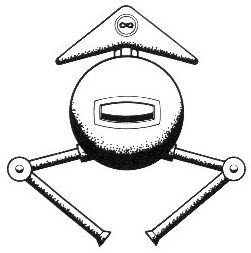
\includegraphics[width=\linewidth]{src/callout/ia.jpg} 
\end{wrapfigure}
\small
Since each tune is dynamically generated there's nowhere for us to pull them from. We could record
the tunes as audio files and maybe extract something useful that way. A feature of Vice, the C64
emulator, allows us to do something much simpler. We can log every note that's played to a 
text file and use that trace to reconstruct the tunes.

We launch Iridis Alpha with \icode{x64} using the following command:

\icode{x64 -moncommands moncommands.txt orig/iridisalpha.prg}

The \icode{moncommands.txt} file contains a series of debugger directives that tells \icode{x64}
to log every value stored to the music registers at \icode{\$D400-\$D415}. This will capture
all notes played on all three voices as well as any updates made to the other sound parameters
and write them to \icode{IridisAlphaTitleMusicAll.txt}:

\begin{lstlisting}[escapechar=\%]
log on
logname "IridisAlphaTitleMusicAll.txt"
tr store D400 D415
\end{lstlisting}

We end up with \icode{IridisAlphaTitleMusicAll.txt} full of lines like:

\begin{lstlisting}[basicstyle=\tiny,escapechar=\%]
TRACE: 1  C:$d400-$d415  (Trace store)
#1 (Trace store d400)  279 052
.C:1598  8D 00 D4    STA $D400      - A:61 X:00 Y:00 SP:e8 ..-..I..   96135469
#1 (Trace store d401)  279 060
.C:159e  8D 01 D4    STA $D401      - A:08 X:00 Y:00 SP:e8 ..-..I..   96135477
#1 (Trace store d40b)  280 059
\end{lstlisting}

This examples gives us the value in \icode{A} written to each register\index{register} for Voice 1. For example, \icode{\$61}
has been written to \icode{\$D400} and \icode{\$08} has been written to \icode{\$D401}.

We can now write a short Python \href{https://github.com/mwenge/iatheory/tree/main/notebooks}{notebook} that
parses this file and for each tune constructs three arrays, each representing a voice, with the sequence\index{sequence}
of notes played to each. For example, in the extract above we can extract \icode{\$0861} as the note 'C'
in octave 3 played on Voice 1 (\icode{\$D400-\$D401}). (Refer to the tables above to see why \icode{\$0861}
translates to 'C-3'.

With the sequence\index{sequence} of notes in three arrays, each representing one of the 3 voices, it is a simple
matter to transform this into ABC format, a music notation frequently used for traditional music.

\lstinputlisting[caption=Title Tune No 1 in ABC format, basicstyle=\tiny]{music/title_no_1_page_1.abc}

We can then use the tool `abcm2ps` to transform this into an SVG image file giving the music in
standard Western notation.

\end{definition}

\subsection{Phrasing}
Now that we've identified the underlying 4-bar structure\index{structure} of the arrangement. We can take a closer look at the 
phrasing of the invidividual parts. Voice 3 has a simple repetitive structure\index{structure} for each 4-bar phrase:

\begin{figure}[H]
{
  \begin{adjustbox}{width=11cm,center}
  \includegraphics[width=11cm]{music/Voice_3_Phrasing1.png}%
    \end{adjustbox}
}\caption[]{Bars 2 and 4 are always repeated}
\end{figure}

Bars 2 and 4 are repeated. Each bar consists of the same tonic formula: three notes rising two notes at a time,
falling back on the final note. The difference between bars 1 and 3 is a simple key change.

This 4 note basis is driven by the 4 bytes in \icode{titleMusicNoteArray\index{titleMusicNoteArray}}. Generating the music for Voice 3
consists of calculating and loading 4 values into this array and using them as an index into  
\icode{titleMusicLowBytes\index{titleMusicLowBytes}}/\icode{titleMusicHiBytes\index{titleMusicHiBytes}} to play the actual note.

\begin{lstlisting}[escapechar=\%]
; This seeds the title music. Playing around with these first
; four bytes alters the first few seconds of the title music.
; The routine%\index{routine}% for the title music uses these 4 bytes to determine
; the notes to play.
; This array is periodically replenished from titleMusicSeedArray%\index{titleMusicSeedArray}% by
; SelectNewNotesToPlay%\index{SelectNewNotesToPlay}%.
titleMusicNoteArray%\index{titleMusicNoteArray}% .BYTE $00,$07,$0C,$07
\end{lstlisting}

Notice how the values populated in \icode{titleMusicNoteArray\index{titleMusicNoteArray}} at start-up match the structure\index{structure} of our basic
tonic formula, e.g. C3-G3-C4-G3.

\begin{figure}[H]
  {
    \setlength{\tabcolsep}{3.0pt}
    \setlength\cmidrulewidth{\heavyrulewidth} % Make cmidrule = 
    \begin{adjustbox}{width=10cm,center}

      \begin{tabular}{rlll}
        \toprule
        \icode{titleMusicNoteArray\index{titleMusicNoteArray}} & \icode{titleMusicHiBytes\index{titleMusicHiBytes}} & \icode{titleMusicLowBytes\index{titleMusicLowBytes}} & Note \\
        \midrule
        \icode{\$00} & \icode{\$08} & \icode{\$61} & C-3 \\
        \icode{\$07} & \icode{\$8F} & \icode{\$0C} & G-3 \\
        \icode{\$0C} & \icode{\$C3} & \icode{\$10} & G-3 \\
        \icode{\$07} & \icode{\$8F} & \icode{\$0C} & G-3 \\
        \bottomrule
      \end{tabular}

    \end{adjustbox}

  }\caption{The value in \icode{titleMusicNoteArray\index{titleMusicNoteArray}} is an index into \icode{titleMusicHiBytes\index{titleMusicHiBytes}/titleMusicLowBytes\index{titleMusicLowBytes}}.}
\end{figure}

Playing the 4 note phrase we've stored in this array is done here:

\begin{lstlisting}[escapechar=\%]
        ; Play the note currently pointed to by 
        ; voice3IndexToMusicNoteArray%\index{voice3IndexToMusicNoteArray}% in titleMusicNoteArray%\index{titleMusicNoteArray}%.
        LDX voice3IndexToMusicNoteArray%\index{voice3IndexToMusicNoteArray}%
        LDA titleMusicNoteArray%\index{titleMusicNoteArray}%,X
        CLC
        ADC offsetForNextVoice3Note%\index{offsetForNextVoice3Note}%
        TAY
        JSR PlayNoteVoice3%\index{PlayNoteVoice3}%

\end{lstlisting}

The variable that's doing a bit of extra work here is \icode{offsetForNextVoice3Note\index{offsetForNextVoice3Note}}. This is what's shifting\index{shifting} the
notes for subsequent bars from the base position of C3-G3-C4-G3 to G3-D4-G4-D4. This value has to get updated after
every four notes, otherwise we just keep playing the same four notes over and over again.

The obvious place to do this is when play a note on Voice 2, which is something we're already doing every 4 notes
in Voice 3.

\begin{lstlisting}[escapechar=\%]
MaybePlayVoice2%\index{MaybePlayVoice2}%   
        DEC voice2NoteDuration%\index{voice2NoteDuration}%
        BNE MaybePlayVoice3%\index{MaybePlayVoice3}%

        LDA #$0C
        STA voice2NoteDuration%\index{voice2NoteDuration}%
        LDX voice2IndexToMusicNoteArray%\index{voice2IndexToMusicNoteArray}%
        LDA titleMusicNoteArray%\index{titleMusicNoteArray}%,X
        CLC
        ADC offsetForNextVoice2Note%\index{offsetForNextVoice2Note}%

        ; Use this new value to change the key of the next four
        ; notes played by voice 3. 
        STA offsetForNextVoice3Note%\index{offsetForNextVoice3Note}%

        TAY
        JSR PlayNoteVoice2%\index{PlayNoteVoice2}%%\index{PlayNoteVoice2%\index{PlayNoteVoice2}%}%
        INX
        TXA
        AND #$03
        STA voice2IndexToMusicNoteArray%\index{voice2IndexToMusicNoteArray}%
\end{lstlisting}

As we can see the mechanics of playing a note for Voice 2 are otherwise the same as Voice 3. We're playing the
same phrase encoded in \icode{titleMusicNoteArray\index{titleMusicNoteArray}} that is played by Voice 3 but just over a longer period of
time. And if you look closely again at the first four bars of the first title tune you can see that Voice 2
is in fact playing the exact same 4 notes of the first bar of Voice 3.

\begin{figure}[H]
{
  \begin{adjustbox}{width=11cm,center}
  \begin{Overpic}[abs,unit=1mm]{%
    \includegraphics[width=11cm]{music/Voice_1_Part.png}}%
      \put(0,0){\color{blue}\linethickness{0.1mm}
        \polygon(15,20)(90,20)(90,10)(15,10)(15,20)}
      \put(0,0){\color{red}\linethickness{0.1mm}
        \polygon(15,9)(35,9)(35,0)(15,0)(15,9)}
    \end{Overpic}
    \end{adjustbox}
  }
  \end{figure}

The same thing happens for Voice 1: it is playing the same notes as the first bar of Voice 3 but over 16 bars (1 every 4 bars).

So ultimately what we have underlying every tune generated by Iridis Alpha is a 16-bar structure\index{structure} where the same 4 notes
are played by Voice 3 in its first bar, Voice 2 in its first 4 bars, and Voice 1 over the full 16 bars. This structure\index{structure} recurs every
16 bars, each time using the 4 initial notes from Voice 3.

\begin{figure}[H]
{
  \begin{adjustbox}{width=11cm,center}
  \includegraphics[width=11cm]{music/16BarStructure_Tune14.png}%
    \end{adjustbox}
}\caption[]{A full 16 bar passage showing the nested structure\index{structure} of Voices 1 and 2}
\end{figure}

This is a nested structure\index{structure} with the initial musical phrase that occurs every 4 bars in Voice 3 being picked up by Voice 2 and the one
that occurs at every 16th bar being picked up by Voice 1.

The second, finer-grained structure\index{structure} of each tune lies in Voice 3 and consists of selecting a fundamental 4 note pattern\index{pattern} (as we 
discussed above) and applying that same pattern\index{pattern} to the key change between each 4 note phrase! 

\begin{figure}[H]
{
  \begin{adjustbox}{width=11cm,center}
  \begin{Overpic}[abs,unit=1mm]{%
    \includegraphics[width=11cm]{music/Tune1_Voice_3_4Bar_Pattern.png}}%

      \put(0,0){\color{red}\linethickness{0.2mm}
        \polygon(8,9)(30,9)(30,0)(8,0)(8,9)}
      \put(0,0){\color{red}\linethickness{0.2mm}
        \polygon(8,20)(30,20)(30,10)(8,10)(8,20)}
      \put(0,0){\color{red}\linethickness{0.2mm}
        \polygon(8,30)(30,30)(30,20)(8,20)(8,30)}
      \put(0,0){\color{red}\linethickness{0.2mm}
        \polygon(8,40)(30,40)(30,30)(8,30)(8,40)}

      \put(0,0){\color{blue}\linethickness{0.2mm}
        \polygon(32,9)(55,9)(55,0)(32,0)(32,10)}
      \put(0,0){\color{blue}\linethickness{0.2mm}
        \polygon(32,20)(55,20)(55,10)(32,10)(32,20)}
      \put(0,0){\color{blue}\linethickness{0.2mm}
        \polygon(32,30)(55,30)(55,20)(32,20)(32,30)}
      \put(0,0){\color{blue}\linethickness{0.2mm}
        \polygon(32,40)(55,40)(55,30)(32,30)(32,40)}

      \put(0,0){\color{green}\linethickness{0.2mm}
        \polygon(58,9)(80,9)(80,0)(58,0)(58,9)}
      \put(0,0){\color{green}\linethickness{0.2mm}
        \polygon(58,20)(80,20)(80,10)(58,10)(58,20)}
      \put(0,0){\color{green}\linethickness{0.2mm}
        \polygon(58,30)(80,30)(80,20)(58,20)(58,30)}
      \put(0,0){\color{green}\linethickness{0.2mm}
        \polygon(58,40)(80,40)(80,30)(58,30)(58,40)}

      \put(0,0){\color{blue}\linethickness{0.2mm}
        \polygon(82,9)(105,9)(105,0)(82,0)(82,10)}
      \put(0,0){\color{blue}\linethickness{0.2mm}
        \polygon(82,20)(105,20)(105,10)(82,10)(82,20)}
      \put(0,0){\color{blue}\linethickness{0.2mm}
        \polygon(82,30)(105,30)(105,20)(82,20)(82,30)}
      \put(0,0){\color{blue}\linethickness{0.2mm}
        \polygon(82,40)(105,40)(105,30)(82,30)(82,40)}

    \end{Overpic}
    \end{adjustbox}
  }\caption[]{The G3-C4-G4-C4 pattern\index{pattern} used to construct the 4 note pattern\index{pattern} is also used to construct the key changes in each 4-bar sequence\index{sequence} (red-blue-green-blue).}
  \end{figure}

This is why we observed the repeating structure\index{structure} of Bars 2 and 4 earlier! It's the same pattern\index{pattern} used to construct the 4 note formula.

But how do we choose the key for
the start of each 4-bar pattern\index{pattern}? By applying the same pattern\index{pattern} to the start of each 4-bar section! 


\begin{figure}[H]
{
  \begin{adjustbox}{width=11cm,center}
  \begin{Overpic}[abs,unit=1mm]{%
    \includegraphics[width=11cm]{music/Tune1_Voice_3_4Bar_Pattern.png}}%

      \put(0,0){\color{blue}\linethickness{0.2mm}
        \polygon(8,9)(30,9)(30,0)(8,0)(8,9)}
      \put(0,0){\color{green}\linethickness{0.2mm}
        \polygon(8,20)(30,20)(30,10)(8,10)(8,20)}
      \put(0,0){\color{blue}\linethickness{0.2mm}
        \polygon(8,30)(30,30)(30,20)(8,20)(8,30)}
      \put(0,0){\color{red}\linethickness{0.2mm}
        \polygon(8,40)(30,40)(30,30)(8,30)(8,40)}

      \put(0,0){\color{blue}\linethickness{0.2mm}
        \polygon(32,40)(55,40)(55,30)(32,30)(32,40)}

      \put(0,0){\color{green}\linethickness{0.2mm}
        \polygon(58,40)(80,40)(80,30)(58,30)(58,40)}

      \put(0,0){\color{blue}\linethickness{0.2mm}
        \polygon(82,40)(105,40)(105,30)(82,30)(82,40)}

    \end{Overpic}
    \end{adjustbox}
  }\caption[]{The start of each 4 bar pattern\index{pattern} in a 16 bar cycle uses each of the 4-note patterns from the first 4 bars.}
  \end{figure}

If we look at two other procedurally\index{procedurally} generated tunes we can see the same pattern\index{pattern}:


\begin{figure}[H]
{
  \begin{adjustbox}{width=11cm,center}
  \begin{Overpic}[abs,unit=1mm]{%
  \includegraphics[width=11cm]{music/Voice_3_Phrasing_Tune12.png}}%
      \put(0,0){\color{blue}\linethickness{0.2mm}
        \polygon(8,9)(30,9)(30,0)(8,0)(8,9)}
      \put(0,0){\color{green}\linethickness{0.2mm}
        \polygon(8,20)(30,20)(30,10)(8,10)(8,20)}
      \put(0,0){\color{blue}\linethickness{0.2mm}
        \polygon(8,30)(30,30)(30,20)(8,20)(8,30)}
      \put(0,0){\color{red}\linethickness{0.2mm}
        \polygon(8,40)(30,40)(30,30)(8,30)(8,40)}

      \put(0,0){\color{blue}\linethickness{0.2mm}
        \polygon(32,40)(55,40)(55,30)(32,30)(32,40)}

      \put(0,0){\color{green}\linethickness{0.2mm}
        \polygon(58,40)(80,40)(80,30)(58,30)(58,40)}

      \put(0,0){\color{blue}\linethickness{0.2mm}
        \polygon(82,40)(105,40)(105,30)(82,30)(82,40)}

    \end{Overpic}
    \end{adjustbox}
}
\end{figure}
\begin{figure}[H]
{
  \begin{adjustbox}{width=11cm,center}
  \begin{Overpic}[abs,unit=1mm]{%
  \includegraphics[width=11cm]{music/Voice_3_Phrasing_Tune18.png}}%
      \put(0,0){\color{blue}\linethickness{0.2mm}
        \polygon(8,9)(30,9)(30,0)(8,0)(8,9)}
      \put(0,0){\color{green}\linethickness{0.2mm}
        \polygon(8,20)(30,20)(30,10)(8,10)(8,20)}
      \put(0,0){\color{blue}\linethickness{0.2mm}
        \polygon(8,30)(30,30)(30,20)(8,20)(8,30)}
      \put(0,0){\color{red}\linethickness{0.2mm}
        \polygon(8,40)(30,40)(30,30)(8,30)(8,40)}

      \put(0,0){\color{blue}\linethickness{0.2mm}
        \polygon(32,40)(55,40)(55,30)(32,30)(32,40)}

      \put(0,0){\color{green}\linethickness{0.2mm}
        \polygon(58,40)(80,40)(80,30)(58,30)(58,40)}

      \put(0,0){\color{blue}\linethickness{0.2mm}
        \polygon(82,40)(105,40)(105,30)(82,30)(82,40)}

    \end{Overpic}
    \end{adjustbox}
}\caption[]{The same patterns in Tunes 12 and 18.}
\end{figure}

\subsection{Seeding the Random}

We've established how each tune is built entirely off the same 4-byte sequence\index{sequence}, all the way from selecting
notes to play to filling out the larger structure\index{structure} of the tune at almost every level. What remains is
to see how this 4-byte sequence\index{sequence} is selected. We know it's not entirely random since if it was, none of us
would ever hear the same tune. 

The selection of our 4-byte structure\index{structure} for each tune happens in \icode{SelectNewNotesToPlay\index{SelectNewNotesToPlay}}. Once a seed
value has been plucked, this is used as an index into \icode{titleMusicSeedArray\index{titleMusicSeedArray}} and the next four values
are populated into our magic 4-byte sequence\index{sequence} that determines everything \icode{titleMusicNoteArray\index{titleMusicNoteArray}}.

\begin{lstlisting}[escapechar=\%,caption=Put a seed byte in the accumulator and multiply this by 4 if it's not zero. This
gives us what we need for the next step.]
SelectNewNotesToPlay%\index{SelectNewNotesToPlay}%
        ; Get a random value between 0 and 15.
        JSR PutProceduralByteInAccumulator%\index{PutProceduralByteInAccumulator}%
        AND #$0F
        ; Jump to InitializeSeedLoop%\index{InitializeSeedLoop}% if it's zero.
        BEQ InitializeSeedLoop%\index{InitializeSeedLoop}%

        ; Otherwise%\index{Otherwise}% multiply it by 4. We do this so that
        ; the 4-byte sequence%\index{sequence}% we choose always starts at
        ; a 4-byte offset in titleMusicSeedArray%\index{titleMusicSeedArray}%.
        TAX
        LDA #$00
MultiplyRandomNumBy4%\index{MultiplyRandomNumBy4}%   
        CLC
        ADC #$04
        DEX
        BNE MultiplyRandomNumBy4%\index{MultiplyRandomNumBy4}%
\end{lstlisting}

\begin{lstlisting}[escapechar=\%,caption=Use our seed value to pull 4 bytes from \icode{titleMusicSeedArray\index{titleMusicSeedArray}} and
store them in \icode{titleMusicNoteArray\index{titleMusicNoteArray}}]
InitializeSeedLoop%\index{InitializeSeedLoop}%   
        ; Put our random number in Y and use it as index into
        ; the seed array.
        TAY
        ; Initialize X to 0, we will use this to iterate up to
        ; 4 bytes for pulling from titleMusicSeedArray%\index{titleMusicSeedArray}%.
        LDX #$00

        ; Pick the first 4 bytes in titleMusicSeedArray%\index{titleMusicSeedArray}% from our
        ; randomly chosen offset and put them in
        ; titleMusicNoteArray%\index{titleMusicNoteArray}%.
MusicSeedArrayLoop%\index{MusicSeedArrayLoop}%   
        LDA titleMusicSeedArray%\index{titleMusicSeedArray}%,Y
        STA titleMusicNoteArray%\index{titleMusicNoteArray}%,X
        INY
        INX
        CPX #$04
        BNE MusicSeedArrayLoop%\index{MusicSeedArrayLoop}%
\end{lstlisting}

\begin{lstlisting}[caption=Our seed bank for 4-byte sequences. It's 64 bytes long\, giving 16 possibles sequences in all.,escapechar=\%]
; This is used to replenish titleMusicNoteArray%\index{titleMusicNoteArray}% with seed valuse
; for the procedurally%\index{procedurally}% generated title screen%\index{screen}% music.
titleMusicSeedArray%\index{titleMusicSeedArray}% .BYTE $00,$03,$06,$08
                    .BYTE $00,$0C,$04,$08
                    .BYTE $00,$07,$00,$05
                    .BYTE $05,$00,$00,$05
                    .BYTE $00,$06,$09,$05
                    .BYTE $02,$04,$03,$04
                    .BYTE $03,$07,$03,$00
                    .BYTE $04,$08,$0C,$09
                    .BYTE $07,$08,$04,$07
                    .BYTE $00,$04,$07,$0E
                    .BYTE $00,$00,$00,$07
                    .BYTE $07,$04,$00,$0C
                    .BYTE $04,$07,$00,$0C
                    .BYTE $07,$08,$0A,$08
                    .BYTE $0C,$00,$0C,$03
                    .BYTE $0C,$03,$07,$00
\end{lstlisting}

The real source of variety here is this 'seed value' that we pluck at the very start of the process.
This is done by \icode{PutProceduralByteInAccumulator\index{PutProceduralByteInAccumulator}} at the very start of \icode{SelectNewNotesToPlay\index{SelectNewNotesToPlay}}.

\begin{lstlisting}[caption= Our seed value ultimately comes from \icode{sourceOfSeedBytes\index{sourceOfSeedBytes}}.,escapechar=\%]
;-------------------------------------------------
; PutProceduralByteInAccumulator%\index{PutProceduralByteInAccumulator}%
; This function%\index{function}% is self-modifying%\index{self-modifying}%. Every time it
; is called it increments the address that
; sourceOfSeedBytes%\index{sourceOfSeedBytes}% points to. Since sourceOfSeedBytes%\index{sourceOfSeedBytes}%
; intially points to $9A00, it will point to $9A01
; after the first time it's called, $9A02 after the
; second time it's called - and so on.
;--------------------------------------------------
PutProceduralByteInAccumulator%\index{PutProceduralByteInAccumulator}%
srcOfProceduralBytes%\index{srcOfProceduralBytes}%   =*+$01
        LDA sourceOfSeedBytes%\index{sourceOfSeedBytes}%
        INC srcOfProceduralBytes%\index{srcOfProceduralBytes}%
        RTS
\end{lstlisting}

And \icode{sourceOfSeedBytes\index{sourceOfSeedBytes}} turns out to be a string of 256 random-looking data at \icode{\$9A00}:

\begin{lstlisting}[caption=Our seed value ultimately comes from \icode{sourceOfSeedBytes\index{sourceOfSeedBytes}}.,escapechar=\%]
*=$9A00
sourceOfSeedBytes%\index{sourceOfSeedBytes}%
        .BYTE $E0,$D3,$33,$1F,$BF,$EC,$EF,$3E
        .BYTE $FA,$70,$DA,$26,$87,$C2,$C9,$9C
        .BYTE $F7,$FB,$C8,$85,$C1,$A9,$64,$AD
        .BYTE $6B,$DE,$8B,$8F,$05,$5E,$54,$51
        .BYTE $78,$0A,$6E,$6F,$FD,$0C,$A5,$32
        .BYTE $F5,$56,$44,$75,$38,$D6,$23,$98
        .BYTE $61,$D5,$49,$C6,$F2,$95,$BA,$08
        .BYTE $C3,$3D,$F4,$F0,$21,$48,$84,$02
        .BYTE $7E,$5B,$68,$55,$04,$92,$AE,$34
        .BYTE $72,$F6,$71,$A1,$39,$4F,$74,$E5
        .BYTE $E8,$31,$9A,$C7,$E3,$86,$6D,$14
        .BYTE $60,$CD,$50,$FF,$82,$52,$66,$9E
        .BYTE $E9,$53,$25,$93,$07,$77,$2E,$D7
        .BYTE $1A,$62,$80,$B7,$0D,$1B,$15,$46
        .BYTE $CE,$AA,$47,$24,$8D,$E1,$18,$67
        .BYTE $6A,$4A,$F1,$B9,$D0,$91,$BC,$EE
        .BYTE $B5,$D1,$7B,$A0,$DB,$36,$45,$E7
        .BYTE $11,$22,$81,$FC,$58,$30,$28,$CB
        .BYTE $8C,$B1,$0B,$A7,$DC,$B4,$9D,$57
        .BYTE $B3,$ED,$3C,$43,$16,$8A,$EA,$D8
        .BYTE $0E,$89,$1D,$1E,$DF,$9F,$BD,$BB
        .BYTE $F9,$D9,$01,$3B,$7A,$BE,$69,$B8
        .BYTE $5A,$A6,$E2,$96,$F8,$AC,$6C,$12
        .BYTE $2D,$19,$2A
\end{lstlisting}

As you might have guessed by now, given that there are only 16 possible sequences to choose from the seed bank there must
actually be a lot less than a hundred thousand billion possible them tunes. With only 16 sequences there may even be
only 16!

Well yes, there are certainly a lot closer to just 16 than a hundred thousand billion. The variety of values we get
from \icode{sourceOfSeedBytes\index{sourceOfSeedBytes}} is not really of any account in the number of tunes we can generate. We're just using it to get pseudo-random but
relatively predicatble values between 0 and 15 and using that to choose one of the 16 4-byte 'tune seeds'.

There's an additional bit of variability that gives us more than just 16 tunes though. This is the value we add to
the note's index before we play it:

\begin{lstlisting}[caption=\icode{offsetForNextVoice1Note\index{offsetForNextVoice1Note}} introduces additional tune permutations.,escapechar=\%]
MaybePlayVoice1%\index{MaybePlayVoice1}%   
        DEC voice1NoteDuration%\index{voice1NoteDuration}%
        BNE MaybePlayVoice2%\index{MaybePlayVoice2}%

        LDA #$30
        STA voice1NoteDuration%\index{voice1NoteDuration}%

        LDX voice1IndexToMusicNoteArray%\index{voice1IndexToMusicNoteArray}%
        LDA titleMusicNoteArray%\index{titleMusicNoteArray}%,X
        CLC
        ADC offsetForNextVoice1Note%\index{offsetForNextVoice1Note}%
        TAY
        STY offsetForNextVoice2Note%\index{offsetForNextVoice2Note}%
\end{lstlisting}

When we select a new tune the value \icode{offsetForNextVoice1Note\index{offsetForNextVoice1Note}} may be carrying over a value from the previous tune so
rather than be a consistent value every time the 'tune seed' is selected, it will vary in value. The result is that the
logic will select a different note-group even though it used the same 4-byte 'tune seed'.

Since the value in \icode{offsetForNextVoice1Note\index{offsetForNextVoice1Note}} is ultimately loaded from \icode{titleMusicSeedArray\index{titleMusicSeedArray}}:

\begin{lstlisting}[escapechar=\%,caption=\icode{offsetForNextVoice1Note\index{offsetForNextVoice1Note}} is loaded from \icode{titleMusicNoteArray\index{titleMusicNoteArray}} and is propagated down
to \icode{offsetForNextVoice3Note\index{offsetForNextVoice3Note}}.]
        LDX notesPlayedSinceLastKeyChange%\index{notesPlayedSinceLastKeyChange}%
        LDA titleMusicNoteArray%\index{titleMusicNoteArray}%,X
        STA offsetForNextVoice1Note%\index{offsetForNextVoice1Note}%
\end{lstlisting}

In practice there are 16 possible voice note sequences and 12 unique possible byte values to load from \icode{titleMusicSeedArray\index{titleMusicSeedArray}}
so there are 192 possible tunes.

[ I can only get it to generate 80 so I'm missing something here.]

So the Hundred Thousand Billion is a lie. Iridis will indeed play a hundred thousand billion times if you 
leave it running long enough but ultimately even when we account for variations in key it can only ever play
192 unique title tunes.

Sorry for getting your hopes up.


